%! suppress = EscapeAmpersand
\section{QUIC in WebRTC}
\label{sec:quic-in-webrtc}
This section outlines how QUIC can be used in WebRTC standard.

\subsection{WebRTC overview}
\label{subsec:webrtc-overview}
WebRTC is a standard that enables peer to peer (P2P) multimedia connections in web browsers when both peers are behind NATs without using any plugins.
It is natively implemented by all major browsers.
In WebRTC there are two planes -- media plane and signaling plane.
The former is responsible for relaying both media data (audio, video) and non-media data (chat messages, uploading and downloading files, etc.).
The later is responsible for negotiating session parameters like audio and video codecs or transport addresses.
The whole protocol stack is presented in figure~\ref{fig:webrtc-stack}.

\begin{figure}[h]
    \centering
    \tikzstyle{rect}=[rectangle,minimum width=6cm,minimum height=1cm,draw=black,outer sep=0pt]
    \tikzstyle{base rect}=[rect,minimum width=12cm,outer sep=0pt]
    \tikzstyle{text rect}=[rectangle,minimum width=6cm,align=center,outer sep=0pt]
    \tikzstyle{multipart rect}=[rectangle split,rectangle split horizontal,rectangle split parts = 2,inner xsep = 0.0mm,outer sep=0pt,
    draw=black,align=center,minimum width=6cm,minimum height=1cm]
    \begin{tikzpicture}
        % ip
        \node (IP) [base rect,fill=gray!20] {IP};

        % media plane
        \node (UDP) [rect,fill=blue!20,above left=0.0cm of IP.north] {UDP};
        \node (ICE) [rect,fill=purple!20,above=0.0cm of UDP]  {ICE, STUN, TURN} ;
        \node (DTLS) [rect,fill=orange!20,above=0.0cm of ICE] {DTLS} ;
        \node (SRTP) [multipart rect,rectangle split part fill={green!20,yellow!20},above=0.0cm of DTLS] {\nodepart[text width=3cm]{one} SRTP \nodepart[text width=3cm]{two} SCTP} ;
        \node [text rect,above=0.0cm of SRTP]{Media Plane};

        % signaling plane
        \node (TCP) [rect,fill=blue!20,above right=0.0cm of IP.north]{TCP};
        \node (TLS) [rect,fill=purple!20,above=0.0cm of TCP] {TLS};
        \node (HTTP) [rect,fill=orange!20,above=0.0cm of TLS] {HTTP};
        \node (WS) [rect,fill=green!20,above=0.0cm of HTTP] {WS/Other};
        \node (SDP) [multipart rect,above=0.0cm of WS,rectangle split part fill={gray!20,yellow!20}] {\nodepart[text width=3cm]{one} SDP \nodepart[text width=3cm]{two} SIP/XMPP/\\Other};
        \node [text rect,above=0.0cm of SDP]{Signaling Plane};
    \end{tikzpicture}
    \caption{WebRTC protocol stack}
    \label{fig:webrtc-stack}
\end{figure}

\subsubsection{Media plane}
\label{subsubsec:media-plane}
In media plane, media data is carried using RTP protocol which stands for Real-time Transport Protocol.
RTP protocol provides media packets with information that is not present in headers of UDP datagrams but is important in terms of multimedia transmission.
This information includes timestamps -- to know when data should be passed to video or audio decoder, sequence numbers -- to perform packets reordering, payload type -- to know which codec is used.
RTP packets are encrypted using cryptographic context negotiated during DTLS handshake.
DTLS handshake provides so called keying material which is used by both sides for creating actual keys used for protecting and unprotecting RTP packets.
Thanks to this we can encrypt only RTP payload (without header) and encapsulate whole RTP packet directly into UDP datagram omitting DTLS record layer.
Key derivation process as well as encryption and decryption mechanisms are described in SRTP (Secure Real-time Transport Protocol) which is a profile of RTP protocol.

On the other hand, non-media data is carried by SCTP\@.
Unlike RTP packets, SCTP datagrams are encapsulated in DTLS datagrams.

Besides SRTP and SCTP protocols there are ICE, STUN and TURN\@.
They are used for establishing a connection between peers even when both of them are behind NATs.

At the end, in most cases everything is carried in UDP datagrams.
However, in some specific scenarios (e.g.\ when some network blocks UDP traffic or allows only for traffic on port 443) TCP or TLS over TCP has to be used.

\subsubsection{Signaling plane}
Main protocol used in signaling plane is Session Description Protocol (SDP).
It defines format of messages that carry information about number of media tracks, their codecs, relationships between them, etc.
WebRTC does not define how to exchange these messages between peers.
Instead, it is user (i.e.\ someone using WebRTC API) responsibility.
In many cases it is done using a separate connection over WebSocket (WS) to a dedicated signaling server.
Figure~\ref{fig:webrtc-architecture} presents WebRTC architecture.

\begin{figure}
    \centering
    \begin{tikzpicture}[node distance = 4cm]
        \node (signaling server)[label=below:{Signaling server}] {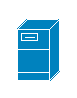
\includegraphics{cisco_icons/fileserver.eps}};

        \node (pc a) [below left=of signaling server,label=below:{PC A}] {
\includegraphics{cisco_icons/workstation.eps}}
        edge [<->, bend left=45] node[align=center,left] {signaling\\messages} (signaling server);
        \node (pc a firewall) [right=0.0cm of pc a,label=below:{NAT}] {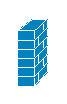
\includegraphics{cisco_icons/firewall.eps}};

        \node (pc b) [below right=of signaling server,label=below:{PC B}] {
\includegraphics{cisco_icons/workstation.eps}}
        edge [<->, bend right=45] node[align=center,right] {signaling\\messages} (signaling server);
        \node (pc b firewall) [left=0.0cm of pc b,label=below:{NAT}] {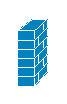
\includegraphics{cisco_icons/firewall.eps}}
        edge [<->] node[above] {audio/video/non-media data} (pc a firewall);

    \end{tikzpicture}
    \caption{WebRTC architecture in P2P scenario}
    \label{fig:webrtc-architecture}
\end{figure}

\subsubsection{Why media plane uses SRTP instead of plain DTLS records}
As stated in section~\ref{subsubsec:media-plane}, RTP packets does not use DTLS record layer.
There are two reasons why.
First of all SRTP protects only RTP payload.
Encapsulating RTP packet in DTLS record would encrypt also RTP header.
The second reason is duplication of data.
Figure~\ref{fig:srtp-packet} illustrates format of an SRTP packet.
Fields that are specific to SRTP profile are \textit{SRTP MKI (Master Key Identifier)} and \textit{authentication tag}.
The rest of fields comes from usual RTP packet.
On the other hand figure~\ref{fig:dtls-packet} presents DTLS record.
We can see that DTLS record includes \textit{sequence number} field that is already in RTP header (they differ only in size) and some other fields like \textit{protocol version} or \textit{epoch}.
Total length of DTLS record header is equal to 104 bits (13 bytes).
All of this data is redundant in terms of multimedia communication.

\begin{figure}
    \centering
    \begin{bytefield}[bitwidth=0.8em]{32}
        \bitheader{0-31} \\
        \begin{rightwordgroup}{\tiny Authenticated \\ \tiny Portion}
            \bitbox{2}{\tiny V=2} & \bitbox{1}{\tiny P} & \bitbox{1}{\tiny X}
            & \bitbox{4}{\tiny CC} & \bitbox{1}{\tiny M} & \bitbox{7}{\tiny PT}
            & \bitbox{16}{\tiny sequence number} \\
            \bitbox{32}{\tiny timestamp} \\
            \bitbox{32}{\tiny synchronization source (SSRC) identifier} \\
            \begin{leftwordgroup}{\tiny 0 to 15 \\ \tiny items}
                \wordbox[tlr]{1}{\tiny contributing source (CSRC) identifiers} \\
                \wordbox[blr]{1}{\tiny $\cdots$}
            \end{leftwordgroup} \\
            \begin{leftwordgroup}{\tiny Optional \\ \tiny RTP \\ \tiny extensions}
                \bitbox{16}{\tiny defined by profile} & \bitbox{16}{\tiny length} \\
                \wordbox[tlr]{1}{\tiny header extension} \\
                \wordbox[blr]{1}{\tiny $\cdots$}
            \end{leftwordgroup} \\
            \begin{leftwordgroup}{\tiny Encrypted \\ \tiny Portion}
                \wordbox[tlr]{2}{\tiny payload} \\
                \bitbox[blr]{16}{} & \bitbox{8}{\tiny RTP padding} & \bitbox{8}{\tiny RTP pad count}
            \end{leftwordgroup}
        \end{rightwordgroup} \\
        \wordbox{1}{\tiny SRTP MKI (OPTIONAL)} \\
        \wordbox{1}{\tiny authentication tag (RECOMMENDED)}
    \end{bytefield}
    \caption{SRTP packet format}
    \label{fig:srtp-packet}
\end{figure}

\begin{figure}
    \centering
    \begin{bytefield}{32}
        \bitheader{0-31} \\
        \bitbox{8}{\tiny type} & \bitbox{16}{\tiny version} & \bitbox{8}{\tiny epoch} \\
        \bitbox{8}{\tiny epoch} & \bitbox{24}{\tiny sequence number} \\
        \bitbox{24}{\tiny sequence number} & \bitbox{8}{\tiny length} \\
        \bitbox{8}{\tiny length} & \bitbox{24}{\tiny fragment} \\
        \wordbox{1}{\tiny fragment}
    \end{bytefield}
    \caption{DTLS packet format}
    \label{fig:dtls-packet}
\end{figure}

\subsection{RTP encapsulation in QUIC}
\label{subsec:rtp-encapsulation-in-quic}
RTP packets should be sent unreliably therefore they must be encapsulated into DATAGRAM frames described in section~\ref{sec:datagrams}.
RTP over QUIC~\cite{engelbart-rtp-over-quic-00} proposes encapsulation presented in figure~\ref{fig:rtp-encapsulation-into-quic-packet}.

\begin{figure}
    \centering
    \begin{bytefield}[bitwidth=3.5em]{8}
        \wordbox{1}{\tiny short header} \\
        \begin{leftwordgroup}{\tiny DATAGRAM \\ \tiny frame}
            \wordbox{1}{\tiny length(i) (OPTIONAL)} \\
            \wordbox{1}{\tiny flow identifier(j)} \\
            \wordbox{1}{\tiny RTP packet}
        \end{leftwordgroup}
    \end{bytefield}
    \caption{RTP encapsulation into QUIC packet}
    \label{fig:rtp-encapsulation-into-quic-packet}
\end{figure}

There are two drawbacks of proposed solution.
The first one is duplication of data as \textit{sequence\_number} field is present both in a QUIC and RTP headers.
The second one is that RTP header will be entirely encrypted as a part of QUIC packet payload.
These caveats are the same as in the case of using DTLS instead of SRTP however, encapsulating RTP in QUIC will result in a much simpler protocol stack.
Comparison of WebRTC protocol stacks is presented in figure ~\ref{fig:webrtc-stack-comparision}

\begin{figure}
    \centering
    \tikzstyle{rect}=[rectangle,minimum width=6cm,minimum height=1cm,draw=black,outer sep=0pt]
    \tikzstyle{text rect}=[rectangle,minimum width=6cm,align=center,outer sep=0pt]
    \tikzstyle{multipart rect}=[rectangle split,rectangle split horizontal,rectangle split parts = 2,inner xsep = 0.0mm,outer sep=0pt,
    draw=black,align=center,minimum width=6cm,minimum height=1cm]
    \begin{subfigure}[b]{0.4\textwidth}
        \begin{tikzpicture}
            % ip
            \node (IP) [rect,fill=gray!20] {IP};

            % media plane
            \node (UDP) [rect,fill=blue!20,above=0.0cm of IP] {UDP};
            \node (ICE) [rect,fill=purple!20,above=0.0cm of UDP]  {ICE, STUN, TURN} ;
            \node (DTLS) [rect,fill=orange!20,above=0.0cm of ICE] {DTLS} ;
            \node (SRTP) [multipart rect,rectangle split part fill={green!20,yellow!20},above=0.0cm of DTLS] {\nodepart[text width=3cm]{one} SRTP \nodepart[text width=3cm]{two} SCTP} ;
        \end{tikzpicture}
        \caption{WebRTC stack.}
        \label{fig:webrtc-stack-comparision-standard}
    \end{subfigure}
    \hfill
    \begin{subfigure}[b]{0.4\textwidth}
        \begin{tikzpicture}
            % ip
            \node (IP) [rect,fill=gray!20] {IP};

            % media plane
            \node (UDP) [rect,fill=blue!20,above=0.0cm of IP] {UDP};
            \node (ICE) [rect,fill=purple!20,above=0.0cm of UDP]  {ICE, STUN, TURN} ;
            \node (QUIC) [rect,fill=orange!20,above=0.0cm of ICE] {QUIC} ;
            \node (RTP) [rect,fill=green!20,above=0.0cm of QUIC] {RTP} ;
        \end{tikzpicture}
        \caption{WebRTC stack with QUIC.}
        \label{fig:webrtc-stack-comparision-quic}
    \end{subfigure}
    \caption{Comparison of current WebRTC protocol stack and alternative WebRTC protocol stack when using QUIC}
    \label{fig:webrtc-stack-comparision}
\end{figure}

\clearpage

\subsection{QUIC packet encryption}
\label{subsec:packet-encryption}
This section outlines encryption process of QUIC packet.
In QUIC not only packet payload is encrypted but also some fields in packet header.

\subsubsection{Payload encryption}
Payload is encrypted using AEAD algorithm.
All cipher-suites used in TLS 1.3 are allowed in QUIC except \textit{AES\_128\_CCM\_8}.
Therefore we have \textit{AES\_128\_GCM}, \textit{AES\_256\_GCM}, \textit{CHACHA20\_POLY1305} and \textit{AES\_128\_CCM}.
Figure~\ref{fig:payload_enc} shows the process of payload encryption.
As a plain text we pass payload and as an associated data we pass plain header.
As a result we get a ciphertext and an authentication tag.

\begin{figure}[h]
    \centering
    \begin{tikzpicture}
        \node (aead) [rectangle, draw=black, minimum width=2cm,minimum height=2cm] {AEAD};
        \node (aead in 0) [rectangle, minimum width=1cm,minimum height=1cm, above left=of aead.south east] {};
        \node (aead in 1) [rectangle, minimum width=1cm,minimum height=1cm, below left=of aead.north east] {};
        \node (payload) [left=3cm of aead in 0] {payload}
        edge [->] node[align=center,above] {plain text} (aead in 0);
        \node (header) [left=3cm of aead in 1] {header}
        edge [->] node[align=center,above] {associated data} (aead in 1);
        \node (cipher text) [align=center, right=3cm of aead] {cipher text + \\ authentication tag}
        edge [<-] node[align=center, above] {output} (aead);
    \end{tikzpicture}
    \caption{QUIC payload encryption scheme}
    \label{fig:payload_enc}
\end{figure}

\subsubsection{Header encryption}
Figure~\ref{fig:header_enc} shows the process of header encryption.
The first step is to get \textit{sample} from encrypted payload.
In most cases a sample is 16 bytes long and it is taken starting from $4 - pn\_len$ byte of encrypted payload.
In the next step the sample is encrypted and its first 5 bytes are taken as mask.
At the end we perform XOR operation on predefined header fields and mask.
As a result we get header with some fields being encrypted.
Algorithm used to encrypt sample depends on negotiated cipher-suite.
For example, if payload is encrypted with AES\_128\_GCM then sample will be encrypted using AES\_128\_ECB\@.

\begin{figure}[h]
    \centering
    \tikzset{XOR/.style={draw,circle, minimum width=1cm, minimum height=1cm, append after command={
    [shorten >=\pgflinewidth, shorten <=\pgflinewidth,]
    (\tikzlastnode.north) edge (\tikzlastnode.south)
    (\tikzlastnode.east) edge (\tikzlastnode.west)}}}
    \begin{tikzpicture}
        \node (xor) [XOR, scale=1.2] {};
        \node (encrypted header) [right=of xor] {encrypted header}
        edge [<-] node[align=center,above] {} (xor);
        \node (mask) [below left=of xor] {mask}
        edge [->, to path={-| (\tikztotarget)}] (xor.south);
        \node (sample) [left=of mask] {sample}
        edge [->] (mask);
        \node (payload) [left=of sample] {payload}
        edge [->] (sample);
        \node (header)  at (payload |- xor) {header}
        edge [->] (xor);
    \end{tikzpicture}
    \caption{QUIC header encryption scheme}
    \label{fig:header_enc}
\end{figure}

\subsection{Tests}
\label{subsec:tests}
Following tests are split into two scenarios.

In the first one I am comparing time needed for encrypting constant length QUIC header (22 bytes) and variable length QUIC payload.
QUIC payload encapsulates RTP packet.
Therefore it consists of constant length flow identifier (1 byte), constant length RTP header (12 bytes) and variable length RTP payload (from 100 to 1200 bytes).

In the second scenario I am comparing time needed for encrypting standalone variable length RTP payload (from 100 to 1200 bytes) and whole QUIC packet which consists of constant length QUIC header (22 bytes) and variable length QUIC payload.
QUIC payload has the same format as in the first test scenario.
Whole QUIC packet size can be obtained from the equation~\ref{eq:quic-packet-size}.
\begin{align}
    \begin{split}
        QUIC\_packet\_size & = RTP\_payload\_size + RTP\_header\_size \\
        & \quad + tag\_identifier + QUIC\_header\_size \\
        & = RTP\_payload\_size + 12 + 1 + 22 \\
        & = RTP\_payload\_size + 35
    \end{split}
    \label{eq:quic-packet-size}
\end{align}

In both test scenarios, encryption process was performed concurrently.

\subsubsection{Environment}
Test environment:
\begin{itemize}
    \item processor: Intel(R) Core(TM) i5-9600K CPU @ 3.70GHz, 6 Cores, 9 MB Cache
    \item memory: 16 GB RAM
    \item operating system: Linux
    \item library: ring 0.16.20
    \item language: Rust
    \item cipher-suite: AES\_128\_GCM
\end{itemize}

\subsubsection{Methodology}
For each RTP payload size following steps were performed:
\begin{itemize}
    \item collect 100 samples
    \item detect and remove outliers
    \item count average from remaining samples
\end{itemize}

\subsubsection{Results}
Figure~\ref{fig:header-payload-enc} presents time comparison between header and payload encryption process.
We can see that QUIC payload encryption time is between 220 and 450 ns.
For 400, 800 and 1200 RTP payload sizes we can observe shorter encryption time than for previous sizes.
This is probably because of concurrent execution of encryption process.
The data can be split across threads in a manner that allocates additional thread for 400, 800 and 1200 bytes.

\begin{figure}[h]
    \centering
    \begin{tikzpicture}
        \begin{axis}[xlabel={RTP payload size (bytes)},
        ylabel={Average time (ns)},
        legend style={legend pos=outer north east}]
            \addplot table[x=size,y=time] {data/quic-header-enc.table};
            \addlegendentry{Header encryption time}
            \addplot table[x=size,y=time] {data/quic-payload-enc.table};
            \addlegendentry{Payload encryption time}
        \end{axis}
    \end{tikzpicture}
    \caption{QUIC header vs QUIC payload encryption time}
    \label{fig:header-payload-enc}
\end{figure}

Figure~\ref{fig:rtp-payload-quic-packet-enc} presents time comparison between RTP payload and QUIC packet (with RTP packet inside) encryption process.
As in the first test scenario, for 400, 800 and 1200 RTP payload sizes we can observe shorter encryption time than for previous sizes.
Encryption of QUIC packet that encapsulates RTP packet is slower by 30--50ns comparing to standalone RTP payload encryption.
This is illustrated in figure~\ref{fig:rtp-payload-quic-packet-enc}.

\begin{figure}[h]
    \centering
    \begin{tikzpicture}
        \begin{axis}[xlabel={RTP payload size (bytes)},
        ylabel={Average time (ns)},
        legend style={legend pos=outer north east}]
            \addplot table[x=size,y=time] {data/quic-packet-enc.table};
            \addlegendentry{QUIC packet encryption time}
            \addplot table[x=size,y=time] {data/rtp-payload-enc.table};
            \addlegendentry{RTP payload encryption time}
        \end{axis}
    \end{tikzpicture}
    \caption{RTP payload vs QUIC packet (with RTP packet inside) encryption time}
    \label{fig:rtp-payload-quic-packet-enc}
\end{figure}

In summary, QUIC header encryption does not introduce a significant overhead for the entire QUIC packet encryption process.
Also, encryption of encapsulated RTP packet into QUIC packet is insignificantly slower than encryption of standalone RTP payload.

%\subsection{SSH}
%Secure Shell protocol allows for secure connections to remote machines over insecure network.
%It defines channels where each channel can be terminal session, forwarded connections etc. \cite{rfc4254}.
%Channels are flow controlled.
%One SSH connection can multiplex multiple SSH channels.
%SSH uses TCP under the hood which is also flow controlled.
%Figure \ref{fig:ssh-connection} presents architecture of SSH connection.
%
%\begin{figure}[h]
%    \begin{subfigure}[b]{0.4\textwidth}
%        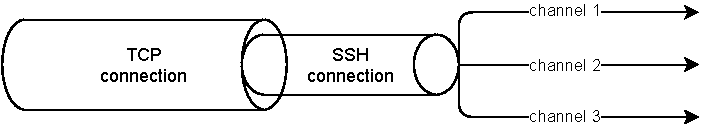
\includegraphics[width=\textwidth]{img/__06__current_standards_and_protocols/ssh.pdf}
%        \caption{SSH connection architecture.}
%        \label{fig:ssh-connection}
%    \end{subfigure}
%    \hfill
%    \begin{subfigure}[b]{0.4\textwidth}
%        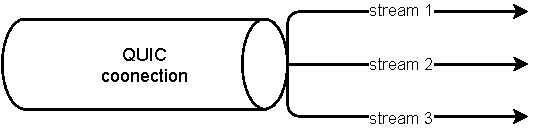
\includegraphics[width=\textwidth]{img/__06__current_standards_and_protocols/quic_ssh.pdf}
%        \caption{Alternative SSH connection architecture with QUIC protocol.}
%        \label{fig:quic-ssh-connection}
%    \end{subfigure}
%    \caption{Comparison of current SSH connection architecture and alternative SSH connection architecture using QUIC protocol.}
%\end{figure}
%
%According to \cite{bider-ssh-quic-09}, using QUIC connection we could remove one level of flow control, reduce connection handshakes from two (one for TCP and one for SSH) to one (only for QUIC) and use streams as SSH channels.
%This approach is presented on figure \ref{fig:quic-ssh-connection}.
